%!TEX root = ../main.tex

\chapter{Non-terrestrial networks}
\label{chp:ntn}
This chapter describes the main charateristics of \ac{NTN}s, i.e., networks where at least one link endpoint is either an aerial or space platform. Specifically, the remainder of this chapter highlights the differences between types of satellites, their advantages and disadvantages as well as the possible choices for payload types. This thesis focuses on the implementation of 5G \ac{NR} in a non-terrestrial scenario, therefore \ac{NR} terminology is used.

\section{Satellite types}
\label{sec:satellite-types}
Satellites are divided in three main different categories, depending on their orbiting altitude: \ac{GEO}, \ac{MEO}, and \ac{LEO} satellites. Each category exhibits has its own characteristics, presenting some upsides and downsides as described in the remainder of this section. Fig. \ref{fig:satellite_coverages} illustrates the different orbiting altitudes as well as estimates of the corresponding coverage areas.

\begin{figure}[ht]
    \centering
    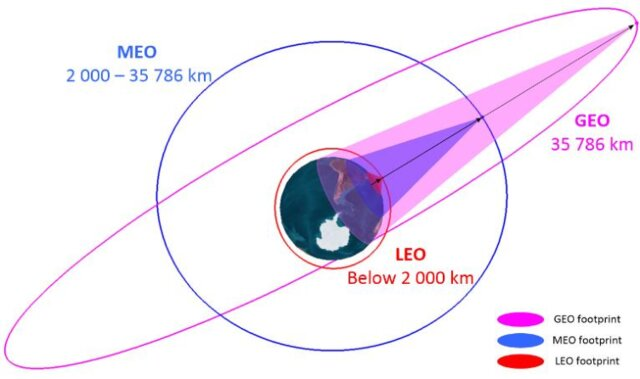
\includegraphics[width=0.9\textwidth]{res/satellite-coverages.jpg}
    \caption{Altitude and approximate coverage areas for satellites at different orbits \cite{sustainable-sat-com-6g}}
    \label{fig:satellite_coverages}
\end{figure}

\subsection{GEO satellites}
Orbiting at an altitude of 35.786Km, to an observer placed on the Earth surface \ac{GEO} satellites appear stationary, since their orbiting period is the same as the Earth rotational period.

\paragraph{Advantages}    
Since \ac{GEO} satellites are geostationary, continuous coverage to a designated area can be provided using as little as a single satellite, while the use of non-\ac{GEO} satellites requires, in general, the deployment of a constellation which is both more complex and more expensive. 

Geostationary satellites also vastly simplify the problem of the ground equipment having to be able to track the satellite. Since the satellite position is always known, once the position of the \ac{UE} is established, the relative position of the satellite can be easily estimated.

As shown in Fig. \ref{fig:satellite_coverages}, the high altitude of \ac{GEO} satellites creates a large cell footprint. Overall, while the deployment cost of a single \ac{GEO} satellite is higher than both \ac{MEO} and \ac{LEO} ones, the cost per coverage area is lower, and an almost full coverage of the terrestrial globe can be achieved using as little as three equally spaced satellites \cite{types-of-orbits-esa}.

\paragraph{Disadvantages}
The disadvantages of \ac{GEO} satellites are mainly caused by their large distance with respect to \ac{UE}s placed on the Earth surface: the transmission power and the antenna gain have to be high enough to overcome the greater propagation losses. Moreover, the propagation delay of the signal increases the baseline latency by approximately 120ms. This means that if the \ac{UE} sends a request to a server at $t=0$ through a \ac{GEO} link, the packet will be received by the destination node at least $t=240$ms. The response will then finally reach the \ac{UE} after at least $480$ms since the initial transmission. These calculations do not factor in any delay related to medium access requests, packet transmission times and processing delays, which would further increase the overall latency.

In addition to the positive aspects previously discussed, the large cell footprint also brings some downsides with it. Due to the vast coverage area, a single satellite will be required to serve a massive number of users. As a consequence, the total available capacity will have to be shared between a bigger number of equipments, and the throughput experienced by each of them will be reduced. Preliminary solutions to overcome this issue comprise, for instance, the use of beamforming to divide the covered area in smaller cells, and the employment of higher frequency bands towards Ku, K and Ka as depicted in Fig. \ref{fig:satellite-bands} \cite{advances-comm-sat-sys}.
Moreover, the high number of users also leads to a large rate of initial access requests, with the possibility of channel saturation as described in \cite{3gpp-tr-38.811}.

\begin{figure}[ht]
    \centering
    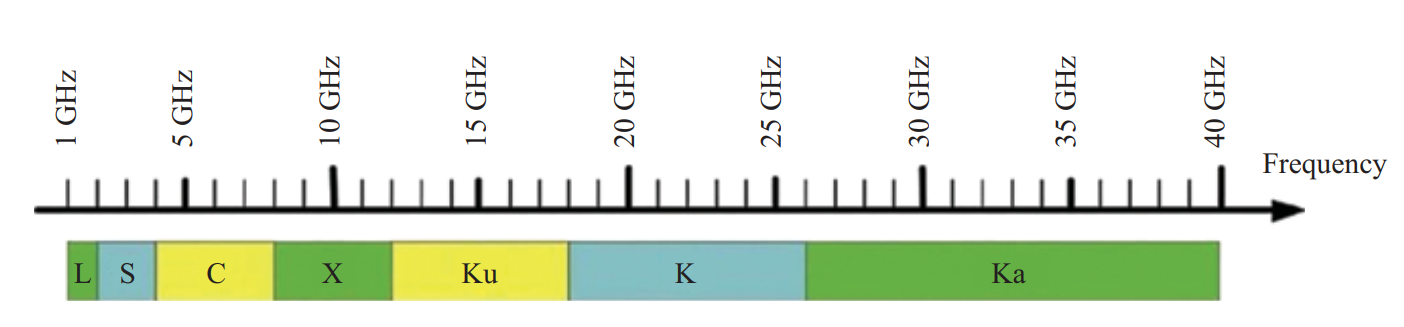
\includegraphics[width=0.9\textwidth]{res/satellite-bands.png}
    \caption{Satellite spectrum bands allocation \cite{advances-comm-sat-sys}}
    \label{fig:satellite-bands}
\end{figure}

\subsection{MEO satellites}
\ac{MEO} orbits sit between the LEO and GEO counterparts. Accordingly, all satellites orbiting between 2000 Km and 35.786 Km are considered as \ac{MEO}. This vast orbital space is mainly used by navigation systems such as GALILEO \cite{types-of-orbits-esa}.

While the propagation delay can vary a lot depending on the altitude, in general it is larger than that of \ac{LEO} and smaller than that of \ac{GEO}. The same point can be made regarding the cell size and number of served users. 

Similarly to \ac{LEO} satellites, \ac{MEO} ones do require a constellation in order to provide continuous coverage over a designated area, since they are not geostationary. Nevertheless, the number of satellites needed for providing continuous coverage is smaller than that required when using \ac{LEO} satellites, since the former can serve a larger area.


Their many downsides in addition to the lack of any substantial benefit over their competitors besides for the need for a smaller constellation makes them less than ideal candidates for applications in \ac{NTN}s.

\subsection{LEO satellites}
\label{sec:leo}
Orbiting below the threshold altitude of 2.000Km, \ac{LEO} satellites represent the most promising solution in the realm of \ac{NTNs}, mainly because they can offer really compelling throughput and propagation delay. However, the latter come at the cost of numerous disadvantages which are peculiar to satellites deployed at this altitude.

\paragraph{Advantages}
The low altitude entails a shorter propagation delay, between 2 and 6 ms. Furthermore, the smaller coverage area of each satellite with respect to \ac{MEO} and \ac{GEO} means that the total number of users that need to be served is smaller. This also enables the use of high frequency bands and the constraints of high antenna gains are less stringent compared to \ac{GEO} satellites, since the experienced path loss is much smaller. In turn, this leads to a higher throughput, more suited to satisfy the requirements of modern days broadband connectivity, as detailed in \cite{satellite-communication-mmwave-giordani}.

The cost per deployed satellite is significantly smaller than that of \ac{GEO} and \ac{MEO} satellites, and multiple deployments within a single launch are possible, further reducing the deployment costs.

\begin{figure}[ht]
    \centering
    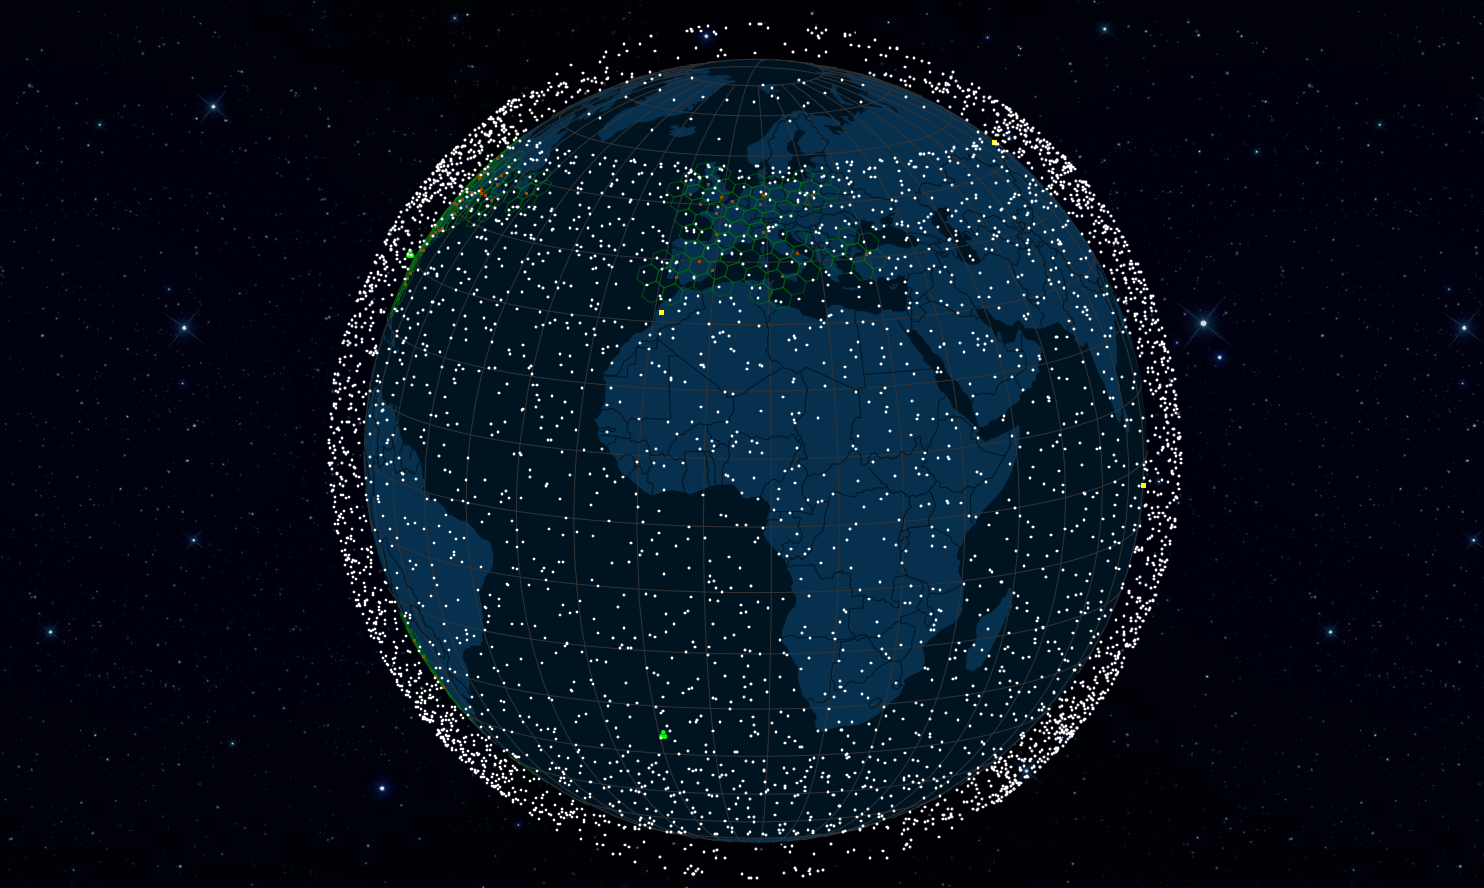
\includegraphics[width=0.9\textwidth]{res/starlink-constellation.png}
    \caption{Starlink constellation as of July 2024. Source: \href{https://satellitemap.space/}{\texttt{satellitemap.space}}}
    \label{fig:starlink_constellation}
\end{figure}

\paragraph{Disadvantages}
Given that \ac{LEO} satellites are not geostationary, a large constellation is needed to provide continuous service, driving the deployment costs significantly up. As an example of how vast those constellations can become, Fig. \ref{fig:starlink_constellation} depicts the \ac{LEO} satellites employed by Starlink\footnote{Starlink is a satellite internet constellation operated by Starlink Services, LLC, a wholly-owned subsidiary of American aerospace company SpaceX.}, counting about 4.808 units in service at the time of writing\footnote{Source: \href{https://satellitemap.space/}{\texttt{satellitemap.space}}}.


Since low orbiting satellites remain view of the \ac{UE}s only for a short period of time, with an average in-view duration of just 13 minutes as calculated in \cite{regional-coverage-analysis-leo}, all the connected users are expected to be handed over to the next available satellite within this time window. Such behavior would create a noticeable protocol overhead, consuming available channel capacity and potentially adding more latency. However, the predictable nature of this phenomenon might allow for a partial automation without requiring explicit control messages to be exchanged.

The small coverage area means that more terrestrial gateways have to be deployed, since each satellite can only communicate with the ground via the terrestrial gateways that fall within its view. A different solution to the densification of gateways is the use of \ac{ISL}, i.e., high-bandwidth links between different satellites of the constellation. The latter are used to connect satellites that do not have gateways in sight to ones that are connected to a gateway, allowing traffic to be routed to the ground via additional hops. Inter-satellite links have also to be implemented if coverage over the oceans is required. Ultimately, this further increases the high constellation deployment costs.

An additional downside affecting all the non-geostationary satellites involves their speed relative to the user equipment located on the ground. A \ac{LEO} satellite moves with a speed of approximately 7.8 km/s \cite{leo-definition-theory-facts}, thus exhibiting a non-negligible Doppler shift. This has to be compensated for, and preliminary solutions in this sense can only be applied to \ac{UE}s which feature GNSS capabilities, which is not always a reasonable assumption \cite{satellite-communication-mmwave-giordani, 3gpp-tr-38.821}. Moreover, the dependency of the network on a third-party service in order to operate properly adds a point of failure which is outside the control of the network operators. Indeed, a disruption in GPS service would halt the network capabilities.

\paragraph{}
The aforementioned advantages make \ac{LEO} satellites the most promising choice in the field of \ac{NTN}s.

\subsection{Multilayered networks}
The aforementioned orbits are not to be considered mutually exclusive. In fact, the multitude of possibilities that their combinations offer opens to the possibility of various different scenario in which the space, air, and ground layers are orchestrated to improve quality of service. An example of such multi-layer network is depicted in Fig. \ref{fig:multilayered-ntn}, showcasing a highly sophisticated non-terrestrial multilayered network scenario where different access technologies are used.

\begin{figure}[ht]
    \centering
    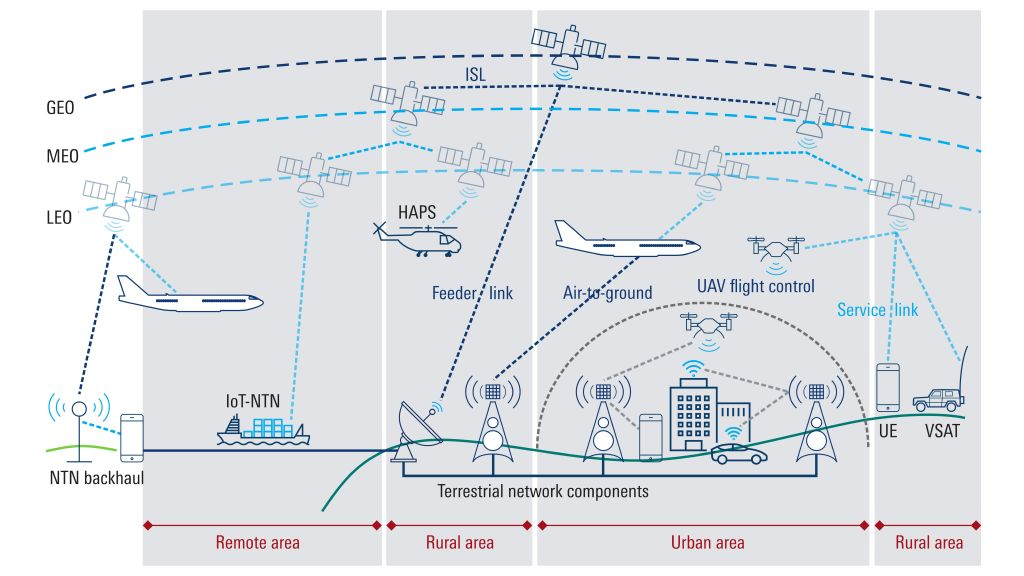
\includegraphics[width=0.9\textwidth]{res/multilayered-ntn.jpg}
    \caption{Complex multilayered \ac{NTN} scenario \cite{connecting-ntn-rohde-schwarz}}
    \label{fig:multilayered-ntn}
\end{figure}

For instance, \cite{potential-multilayered-nierarchical-ntn-wang} argues that that the use of \acp{HAP} as relays between the ground segment of the network and the upper \ac{GEO} satellite links can deliver up to six times the capacity, and better overall outage probability, than point-to-point \ac{GEO} transmissions.


\section{Types of payloads}
When implementing a \ac{NTN}, an important choice to be made is the type of payload to use. There are two main categories: bent-pipe payload and on-board \ac{gNB}. Each one has its own benefits as briefly described below.

\subsection{Bent-pipe payload}
\label{sec:bent-pipe-payload}
This is the simplest approach, where the role of the satellite consists only of  repeating the signal received from the \ac{UE} on the ground towards the terrestrial gateway. Configurations such as the one depicted in Fig. \ref{fig:ntn-bent-pipe} go by the name of bent pipe payloads and are characterized by the presence of a terrestrial g-NodeB, while the satellite has the sole purpose of providing a transparent link to the \ac{UE}.

While such solutions are by far the simplest in terms of payload complexity, the main drawback is the even longer experienced latency. Since communications between users served by the same satellite would also have to be routed through the terrestrial gateway, the overall latency increases by at least two times the propagation delay.
This solution also poses strict bandwidth requirements on the feeder link, since all the traffic must necessarily pass through it.
More complex solutions are able to route at least part of the inbound traffic autonomously, without routing everything back to earth.

\begin{figure}[ht]
    \centering
    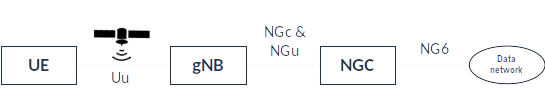
\includegraphics[width=0.9\textwidth]{res/ntn-bent-pipe.png}
    \caption{5G NR NTN architecture for access network based on satellites with bent pipe payload \cite{3gpp-tr-38.811}}
    \label{fig:ntn-bent-pipe}
\end{figure}

\subsection{On-board g-NodeB}
\label{sec:onboard-gnb}
A slightly more sophisticated approach foresees the installation of g-NodeB capabilities directly onto the satellite payload, as depicted in Figure \ref{fig:ntn-gnb-onboard}. This has the benefit of reducing the experienced latency, as well as reducing the utilization of the feeder link. Certain protocols, designed to terminate at the \ac{gNB}, can in this case reach their designated endpoint without necessitating to be routed back to the ground gateway.

\begin{figure}[ht]
    \centering
    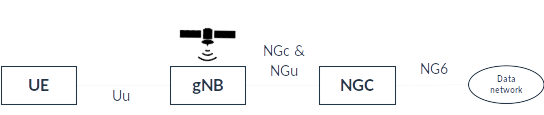
\includegraphics[width=0.9\textwidth]{res/ntn-regen.png}
    \caption{5G NR NTN architecture for access network based on satellites with on-board gNB payload \cite{3gpp-tr-38.811}}
    \label{fig:ntn-gnb-onboard}
\end{figure}

\section{Commercial solutions}
\paragraph{Legacy solutions}
Commercial solutions, initially concerning satellite-based phone calls and successively evolved to provide Internet access, have been available dating back to 2003, when the first Internet satellite was launched \cite{first_internet_sat}. However, the majority of this legacy infrastructure makes use of \ac{GEO} satellites, therefore presenting all the limitations discussed in section \ref{sec:satellite-types}, i.e., they offer limited throughput and large delays. Such constraints render this technology not suitable for the needs of modern internet connections standards.

\paragraph{Recent developments}
Commercial solutions which make use of \ac{LEO} satellites are starting to appear, and they are experiencing moderate commerical success. Notable examples are Starlink and Eutelsat OneWeb. However, these solutions make use of proprietary protocols. Until now, no internationally agreed standard has been defined. This is where most of the research is currently being conducted and where the business world is posing its attention due to the characteristics of \ac{LEO} satellites that makes them the most suited to provide high speed satellite internet access.